\section{Примера работы программы}

На рисунка \ref{fig:code} и \ref{fig:result} предствален код программы с детальным описание каждой строки и результат программы соответсвенно

\begin{figure}[h]
	\centering
	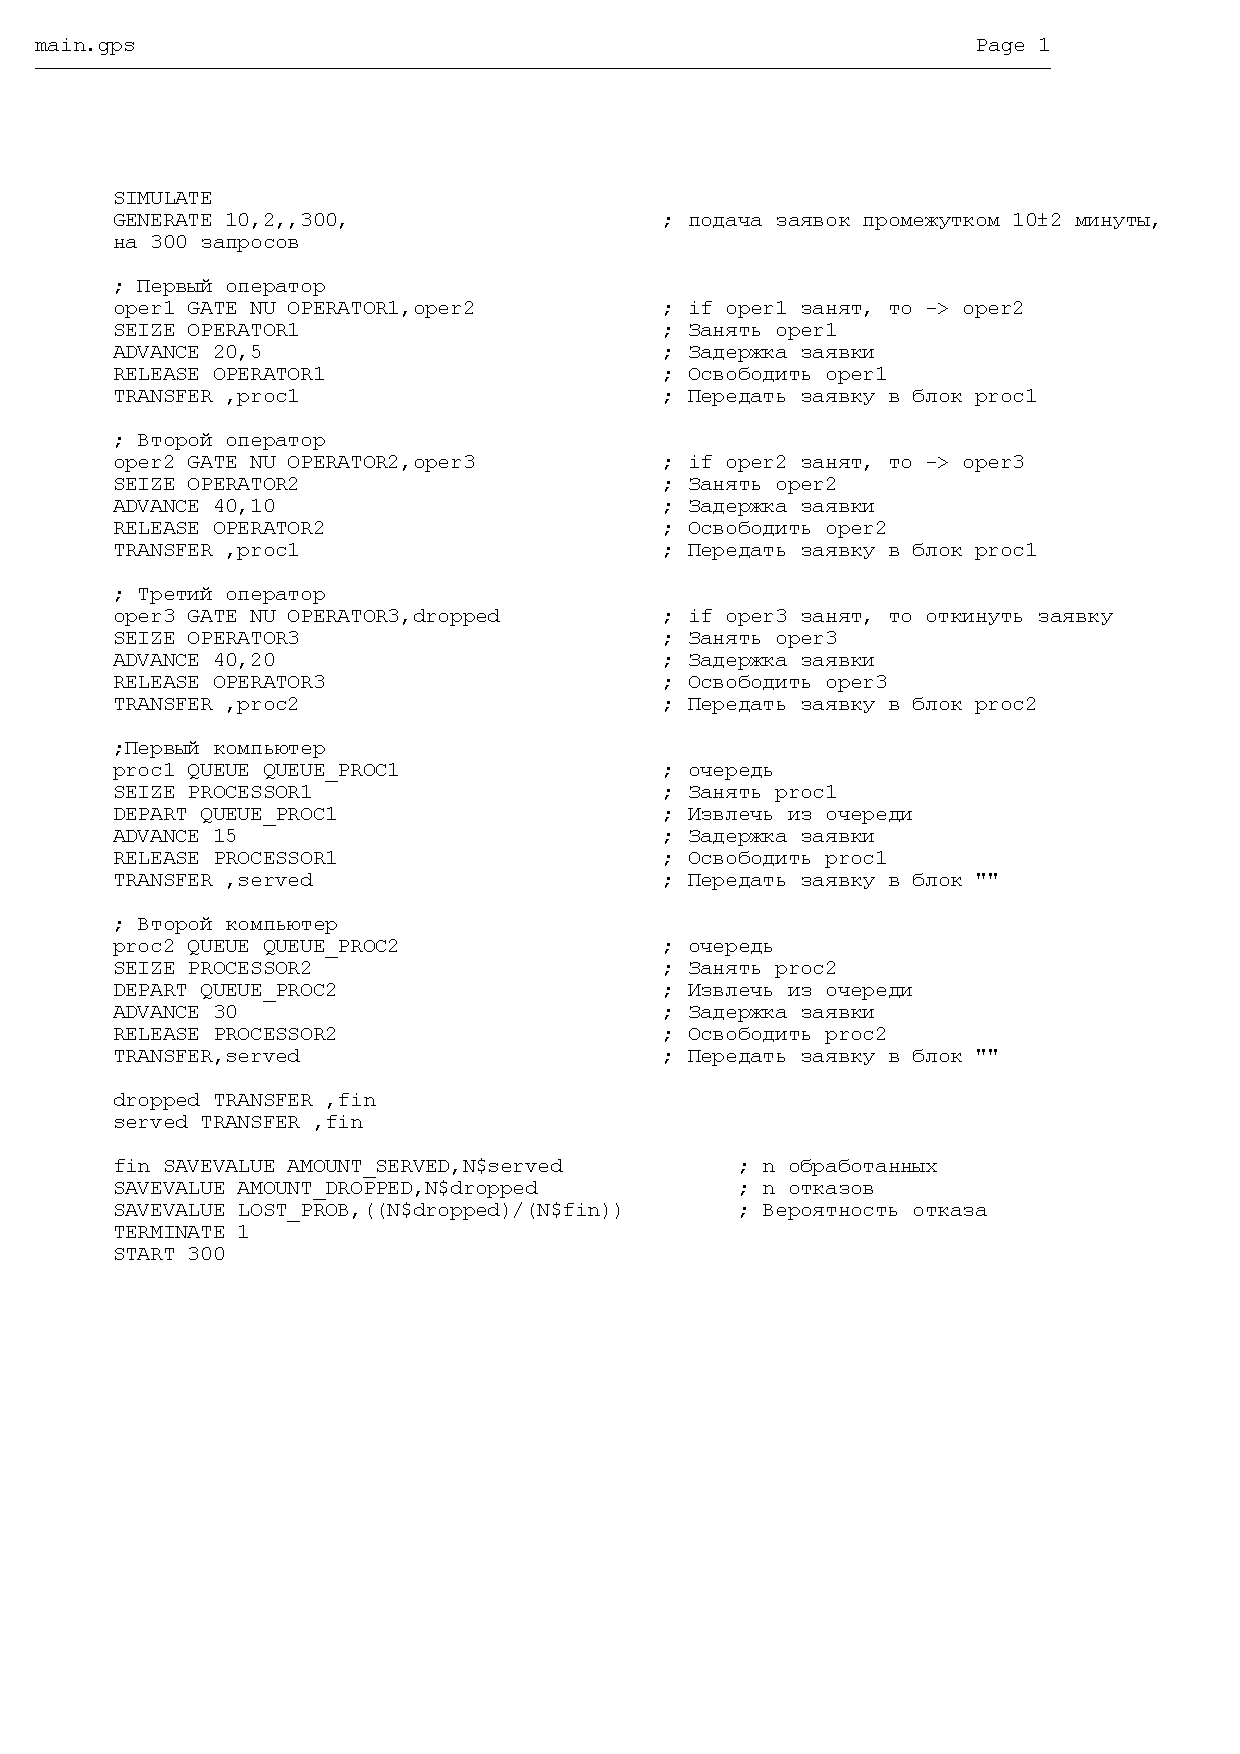
\includegraphics[width=0.7\linewidth]{src/code}
	\caption{Код}
	\label{fig:code}
\end{figure}

\begin{figure}[h]
	\centering
	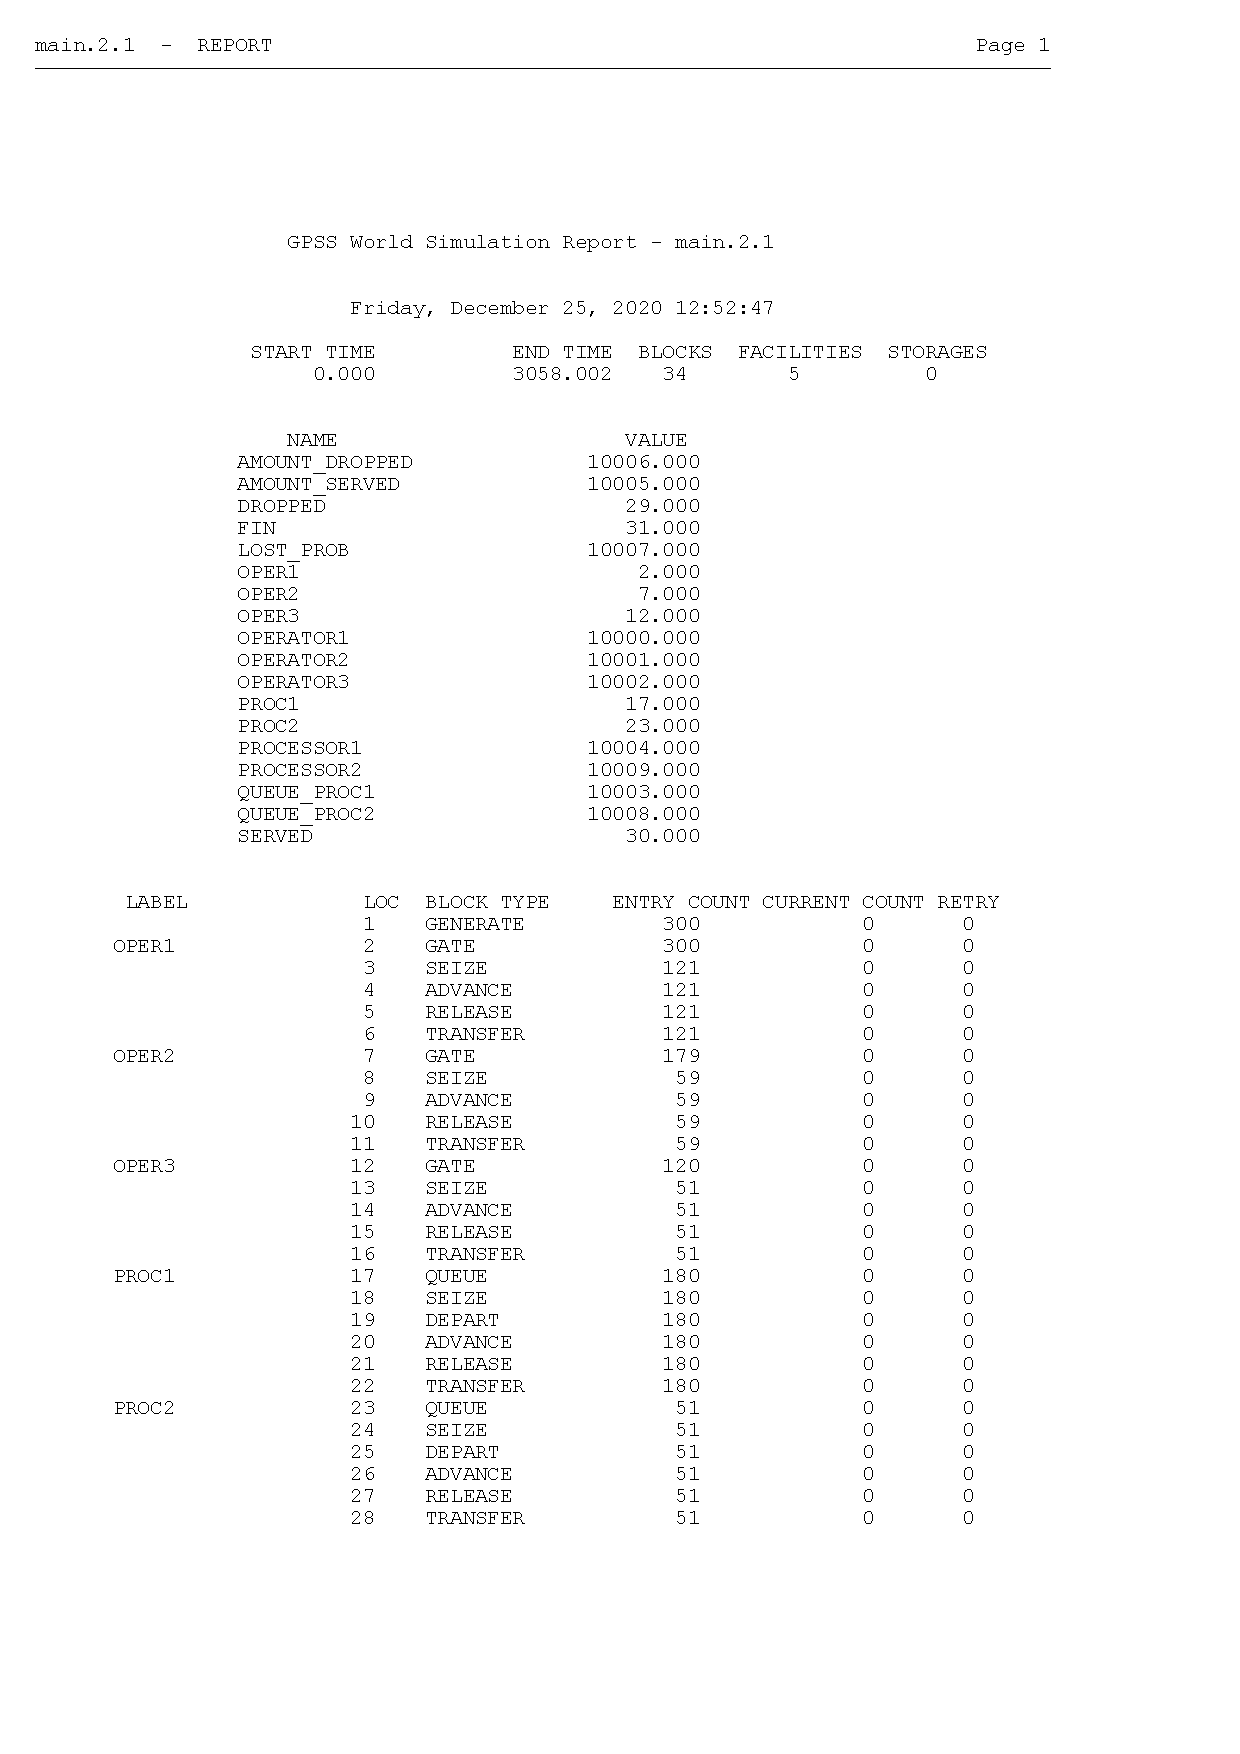
\includegraphics[width=0.7\linewidth]{src/result}
	\caption{Вывод программы}
	\label{fig:result}
\end{figure}


При множественном прогоне среднея вероятность отказа составляет 0.2.